\documentclass[11pt, a4paper]{article}

\usepackage[top=2cm, bottom=2.2cm, left=2.2cm, right=2.2cm]{geometry}
\usepackage[T1]{fontenc}
\usepackage{lmodern}
\usepackage{microtype}
\usepackage{booktabs}
\usepackage{graphicx}
\usepackage{caption}
\usepackage[hidelinks]{hyperref}
\usepackage{titlesec}
\usepackage{fancyhdr}
\usepackage{float}

\setlength{\parskip}{3pt}
\setlength{\parindent}{0pt}

\captionsetup{font=small, labelfont=bf, skip=3pt, belowskip=-6pt}

\titleformat{\section}{\normalfont\small\bfseries\uppercase}{}{0em}{}
  [\vspace{1pt}\titlerule\vspace{2pt}]
\titlespacing{\section}{0pt}{8pt}{3pt}

\titleformat{\subsection}{\normalfont\small\itshape}{}{0em}{}
\titlespacing{\subsection}{0pt}{4pt}{1pt}

\pagestyle{fancy}
\fancyhf{}
\renewcommand{\headrulewidth}{0.4pt}
\fancyhead[L]{\small\textit{Mesa Framework Assessment}}
\fancyhead[R]{\small\textit{PolicySim}}
\fancyfoot[C]{\small\thepage}

\begin{document}

\thispagestyle{empty}
\begin{center}
  {\Large\bfseries Mesa Framework Assessment}\\[3pt]
  {\small PolicySim --- Labour-Market Displacement Prototype}\\[2pt]
  \rule{\linewidth}{0.5pt}
\end{center}

\vspace{2pt}

\section{Benchmark results}

\begin{table}[H]
\centering
\setlength{\tabcolsep}{14pt}
\begin{tabular}{lrr}
\toprule
\textbf{Population} & \textbf{Mean tick} & \textbf{p95 tick} \\
\midrule
10,000    & 1.77 ms      & 2.43 ms  \\
100,000   & 17.57 ms     & 19.13 ms \\
1,000,000 & $\sim$175 ms & ---      \\
\bottomrule
\end{tabular}
\caption{Vectorised, 10 ticks, \texttt{seed = 42}. Two runs: bit-for-bit identical.}
\label{tab:benchmarks}
\end{table}

\section{Assessment}

\subsection{Scale}
Near-linear to 300K (Figure~\ref{fig:scaling}); at 1M, $\sim$175 ms per tick.
Mesa's default per-agent loop would push that past 500 ms.
\textit{Verdict: Mesa's scheduler does not hold up at 1M+ agents; the O($N$) Python loop is the bottleneck, not the underlying maths.}

\begin{figure}[H]
  \centering
  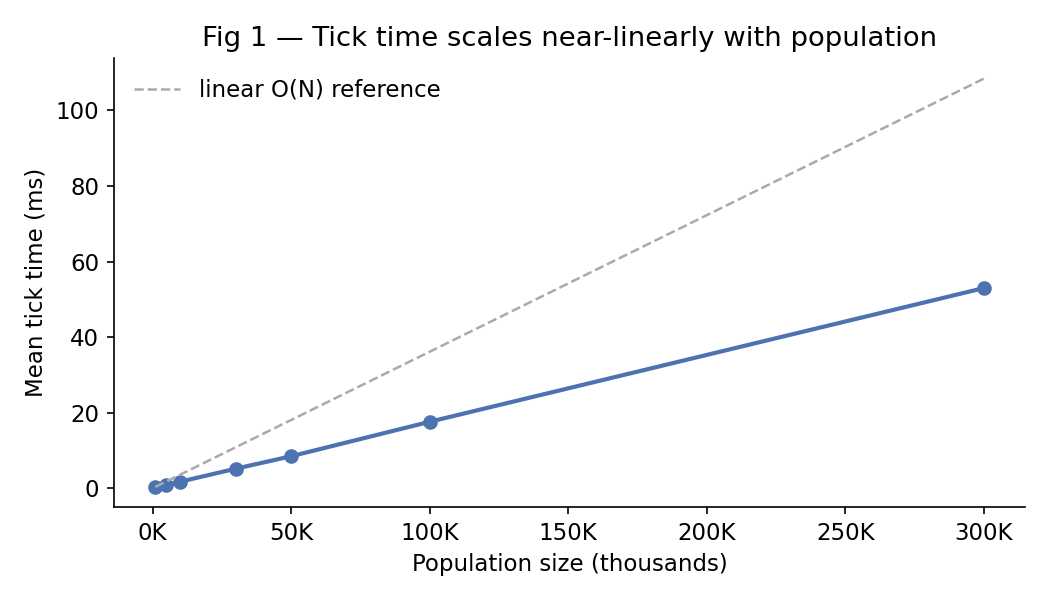
\includegraphics[width=0.70\textwidth]{fig1_scaling.png}
  \caption{\textbf{Figure 1} --- Tick time vs.\ population, 1K--300K agents.}
  \label{fig:scaling}
\end{figure}

\subsection{Aggregate feedback}
Three lines implement it; Figure~\ref{fig:feedback} confirms it works.
Mesa has nothing built in for population-level feedback.
\textit{Verdict: Mesa's architecture is optimised for local agent-to-agent interaction; population-level aggregation requires entirely manual plumbing.}

\begin{figure}[H]
  \centering
  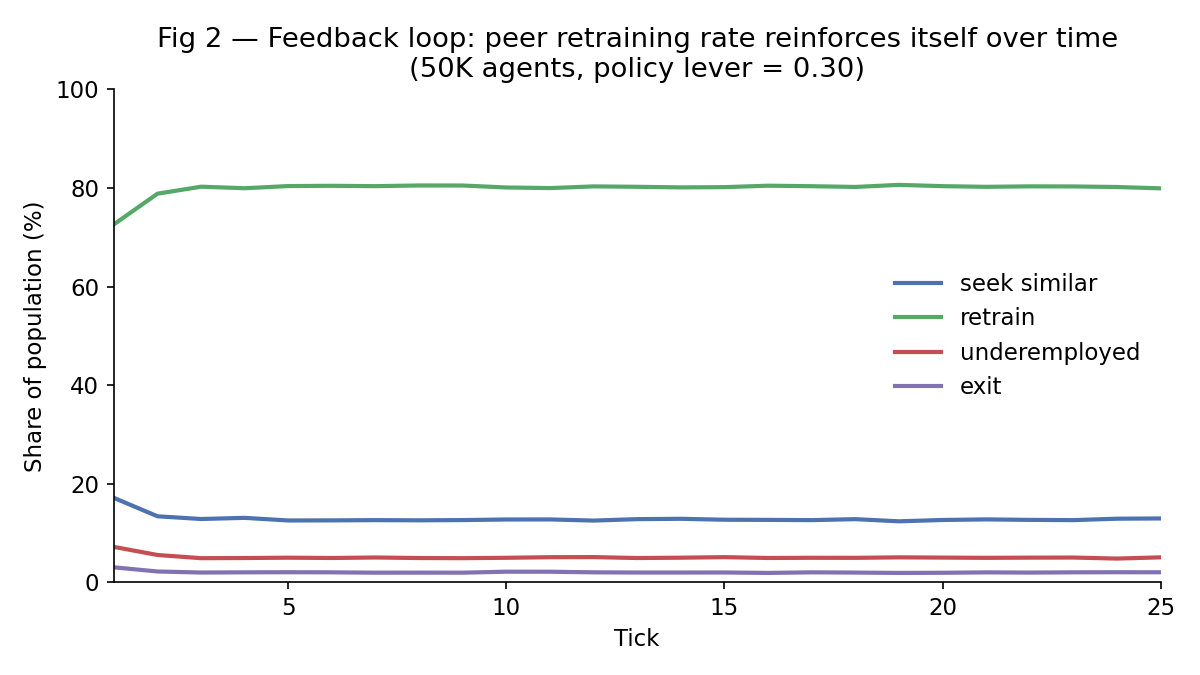
\includegraphics[width=0.70\textwidth]{fig2_feedback_loop.png}
  \caption{\textbf{Figure 2} --- Outcome shares over 25 ticks, 50K agents.}
  \label{fig:feedback}
\end{figure}

\subsection{Parameter sweeps}
\texttt{batch\_run()} works at this scale; \texttt{multiprocessing.Pool}
is faster for larger sweeps (Figure~\ref{fig:sweep}).
\textit{Verdict: Adequate for moderate sweeps; for production-scale parameter searches, Mesa's overhead is unnecessary.}

\begin{figure}[H]
  \centering
  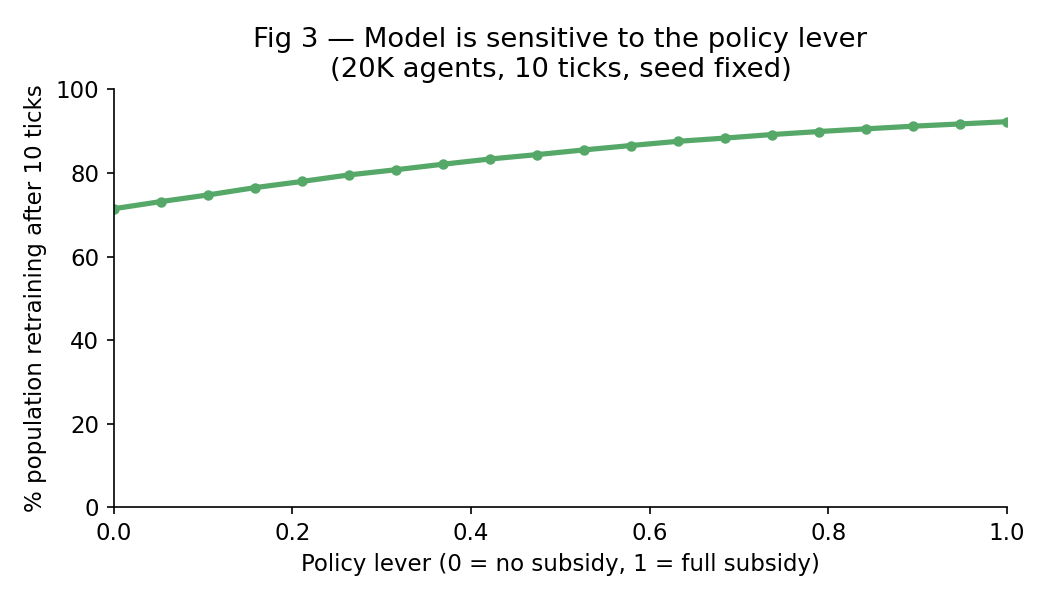
\includegraphics[width=0.70\textwidth]{fig3_policy_sweep.png}
  \caption{\textbf{Figure 3} --- Retraining share vs.\ policy lever, 20 values.}
  \label{fig:sweep}
\end{figure}

\subsection{Vectorisation}
Per-agent \texttt{step()} fights the matrix multiply; the prototype leaves it
empty and runs the population as one NumPy operation. Figure~\ref{fig:writeback}
shows the cost: 63\% overhead at 300K agents (52 ms vs.\ 32 ms).
\textit{Verdict: Mesa's per-agent paradigm is fundamentally misaligned with vectorised multinomial logit; the two cannot coexist without paying a measurable performance penalty.}

\begin{figure}[H]
  \centering
  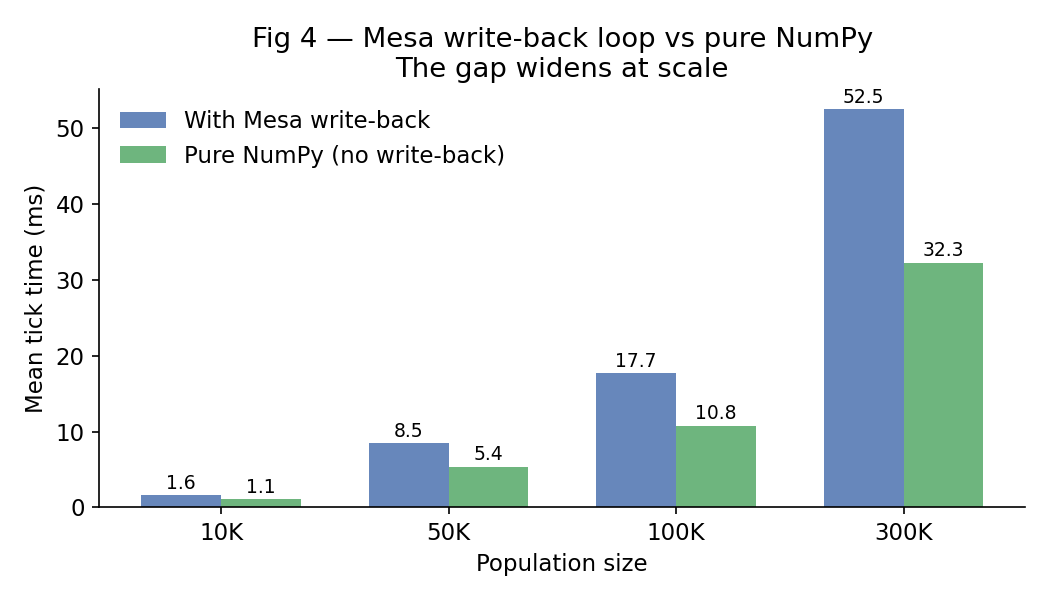
\includegraphics[width=0.70\textwidth]{fig4_writeback_cost.png}
  \caption{\textbf{Figure 4} --- Mesa write-back vs.\ pure NumPy.}
  \label{fig:writeback}
\end{figure}

\subsection{Reproducibility}
Single \texttt{default\_rng(seed)} makes it trivial; two runs with
\texttt{seed = 42} came out identical (Table~\ref{tab:benchmarks}).
\textit{Verdict: Mesa adds no complexity here; reproducibility is a property of the RNG, not the framework.}

\subsection{Data collection}
A 50-run sweep at 1M agents needs 20 GB; \texttt{DataCollector}
holds everything in memory and has no streaming.
\textit{Verdict: DataCollector is unsuitable at this scale; production runs require a custom streaming aggregator writing to disk per tick.}

\subsection{Generality}
Around 30 lines change per domain swap; the engine, seeding, and
benchmark harness stay the same.
\textit{Verdict: Mesa's Model/Agent abstraction is genuinely domain-agnostic; this is its strongest technical argument.}

\section{Recommendation}

Don't run production sweeps on Mesa. The write-back loop adds 40--60\%
overhead at 100K+ agents and \texttt{DataCollector} breaks at scale.
Prototype in Mesa; run production as a standalone NumPy engine on the
same config files.

\medskip
\noindent Mesa is the whiteboard. NumPy is the engine.

\end{document}
